\documentclass{article}

% Paquetes para mejor apariencia y personalización
\usepackage{amsmath}
\numberwithin{equation}{section}
\usepackage[utf8]{inputenc}  % Codificación de caracteres
\usepackage{graphicx}        % Incluir imágenes
\usepackage{imakeidx}
\makeindex[options=-c, intoc]


\title{MÉTODOS DE DETERMINACIÓN DE ÓRBITAS A PARTIR DE OBSERVACIONES}   % Título del artículo
\author{
    Víctor Ávila Camargo, José Ignacio Miguel Rodríguez, Javier Zaragozano Calvo
}
\date{\today}  % Fecha del artículo, por defecto pone la fecha actual.

\begin{document}

% Generar la portada
\maketitle
%\includegraphics[width=1\textwidth]{portada.jpg}
\newpage

\tableofcontents

\newpage

\begin{abstract}
    En este artículo se abordarán varios métodos para determinar 
    las órbitas de cuerpos celestes a partir de obervaciones 
    proporcionadas por la NASA.
\end{abstract}
\newpage
\section{Introducción} %Motivación del problema
\index{Introducción}
Hoy en día y desde hace ya un tiempo, cada día se descubren 
varios exoplanetas cada uno con sus propias características. 
Para terminar de caracterizarlos por completo, es necesario 
hacer un estudio de cómo es su órbita. Esto es bastante 
importante porque estudiando su órbita podemos estimar algunos 
datos sobre ese exoplaneta que de otro modo sería imposible. 
Un ejemplo sería ver si se encuentra en la zona habitable 
o no de su estrella viendo qué tan grande es el periodo de su 
órbita. \\

Sin embargo, tomar una medida de su posición cada día sería 
algo tremendamente ineficiente. Es por eso que antiguos 
matemáticos y físicos desarrollaron algunos métodos para 
determinar su órbita de manera preliminar a partir de, generalmente, 
tres medidas. Algunos de estos métodos son el método de 
Gauss o el método de Gibbs. \\

Estos métodos han logrado varios hitos bastante importantes 
en la historia de la mecánica celeste. Uno de estos logros 
y quizás el más importante fue la determinación de la órbita 
del planeta enano Ceres. Este palneta enano fue descubierto 
el 1 de enero de 1801 por el astrónomo italiano Giuseppe Piazzi ($1746-1826$). 
Sin embargo, debdio a su rápido movimiento, pronto le perdieron 
de vista y ahí es cuando aparece el matemático Carl Friedrich Gauss ($1777-1855$) 
que, con su método, calculó la órbita de Ceres a partir de 
las pocas observaciones que había de él en la época y, gracias 
a su alta precisión, pudieron volver a localizarle. \\

Una vez motivado el esfuerzo de dedicarle un artículo a los 
método de determinación de órbitas, vamos a comenzar desarrollando 
el aspecto más teórico de los tres métodos en los que nos 
vamos a centar: El método de Gauss, el método de Gibbs y 
el método %El posible último método
\section{Método de Gibbs}
\index{Método de Gibbs}
Para este método es necesario conocer la posición de un cuerpo 
respecto a la Tierra en 3 instantes de tiempo distintos, 
$t_{1}$, $t_{2}$ y $t_{3}$. A partir de estas tres posiciones, 
podremos obtener las velocidades $\overrightarrow{v_{1}}$, 
$\overrightarrow{v_{2}}$ y $\overrightarrow{v_{3}}$ suponiendo 
que nos encontramos en una órbita de dos cuerpos. La solución a 
este problema la obtuvo el americano J.W. Gibbs ($1839-1903$) 
usando simplemente un análisis vectorial. A continuación, 
entraremos más en detalle sobre cómo se deduce este método.
\subsection{Deducción del método de Gibbs}
Nosotros sabemos que, por la conservación del momento angular, 
las posiciones de un cuerpo que orbita a otro se encuentran todas 
en el mismo plano. Entonces, partiendo de nuestras tres posicones 
obtenidas en tres tiempos distintos, podemos calcular el 
vector unitario de $\overrightarrow{r_{1}}$ y otro vector 
unitario que sea resultado del producto vectorial de $r_{2}$ y 
$r_{3}$ del siguiente modo: 
\begin{align*}
    &\hat{u}_{r1}=\frac{\overrightarrow{r_{1}}}{r_{1}} \\
    &\hat{C}_{23}=\frac{\overrightarrow{r_{2}}\times \overrightarrow{r_{3}}}{\left\lVert \overrightarrow{r_{2}}\times \overrightarrow{r_{3}} \right\rVert }  
\end{align*}
Como $\overrightarrow{r_{1}}$, $\overrightarrow{r_{2}}$ y 
$\overrightarrow{r_{3}}$ están en el mismo plano, entonces: 
\begin{equation*}
    \hat{u}_{r1}\cdot \hat{C}_{23}=0
\end{equation*}
Además, como se ve en la siguiente figura, nosotros podemos 
expresar $\overrightarrow{r_{2}}$ como una combinación lineal 
de $\overrightarrow{r_{1}}$ y $\overrightarrow{r_{3}}$: 
\begin{equation}
    \overrightarrow{r_{2}}=\alpha \overrightarrow{r_{1}}+\beta \overrightarrow{r_{3}}
\end{equation}
\begin{figure}[h]
    \centering
    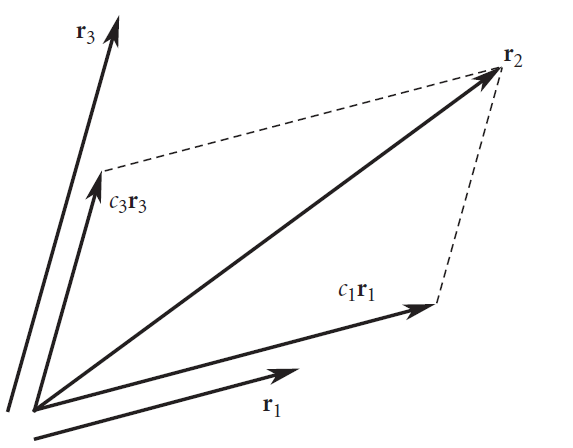
\includegraphics[width=0.6\textwidth]{a.png}
    \caption{Demostración de la ecaución 2.1 (Créditos 
    HowardD. Curtis)}
\end{figure} \\

Una vez tenemos estas consideraciones en mente ya podemos 
empezar a calcular las distintas velocidades. \\

Para calcular las velocidades vamos a partir de la siguiente 
fórmula: 
\begin{equation}
    \overrightarrow{v}\times \overrightarrow{h}=\mu\left(\frac{\overrightarrow{r}}{r}+\overrightarrow{e}\right) 
\end{equation}
Donde $\overrightarrow{h}$ es el momento angular y 
$\overrightarrow{e}$ es el vector excentricidad. Para despejar 
$\overrightarrow{v}$ vamos a multiplicar vectorialmente a ambos 
lados por $\overrightarrow{h}$. Entonces, centrándonos de momento 
en lado izquierdo de la ecuación, obtenemos: 
\begin{equation*}
    \overrightarrow{h}\times(\overrightarrow{v}\times\overrightarrow{h})
\end{equation*}
Para continuar vamos a aplicar la siguiente propiedad del 
triple producto vectorial: $\overrightarrow{A}\times(\overrightarrow{B}\times\overrightarrow{C})
=(\overrightarrow{A}\cdot\overrightarrow{C})\overrightarrow{B}-(\overrightarrow{A}\cdot\overrightarrow{B})\overrightarrow{C}$
y obtenemos lo siguiente: 
\begin{equation*}
    \overrightarrow{h}\times(\overrightarrow{v}\times\overrightarrow{h})=(\overrightarrow{h}\cdot\overrightarrow{h})\overrightarrow{v}-(\overrightarrow{v}\cdot\overrightarrow{h})\overrightarrow{h}
\end{equation*}
Pero como $\overrightarrow{h}\cdot\overrightarrow{h}=h^{2}$ y 
$\overrightarrow{v}\perp\overrightarrow{h}$ obtenemos: 
\begin{equation*}
    \overrightarrow{h}\times(\overrightarrow{v}\times\overrightarrow{h})=h^{2}\overrightarrow{v}
\end{equation*}
Y nuestra ecaución 2.2 queda de la siguiente manera:
\begin{equation}
    \overrightarrow{v}=\frac{\mu}{h^{2}}\left(\frac{\overrightarrow{h}\times\overrightarrow{r}}{r}+\overrightarrow{h}\times\overrightarrow{e}\right)
\end{equation}
Cabe destacar que, en el sistema perifocal, el vector unidad 
$\hat{p}$ tiene la misma dirección que el vector 
de la excentricidad y el vector $\hat{w}$ es perpendicular 
al plano de la órbita en la dirección de $\overrightarrow{h}$. Por 
lo que, en el sistema perifocal, nuestra ecuación se transforma en: 
\begin{equation}
    \overrightarrow{v}=\frac{\mu}{h^{2}}\left(\frac{h\hat{w}\times\overrightarrow{r}}{r}+h\hat{w}\times e\hat{p}\right)=\frac{\mu}{h}\left[\frac{\hat{w}\times\overrightarrow{r}}{r}+e(\hat{w}\times\hat{p})\right]
\end{equation}
Como $\hat{w}$ y $\hat{p}$ son 2 vectores 
de la base en el sistema perifocal, entonces su producto 
vectorial será el tercer vector de la base ($\hat{q}$). 
Así que esto hace que nuestra ecuación se reduzca a: 
\begin{equation}
    \overrightarrow{v}=\frac{\mu}{h}\left(\frac{\hat{w}\times\overrightarrow{r}}{r}+e\hat{q}\right)
\end{equation}
Este es un resultado muy importante porque nos marca nuestro 
camino a seguir. Necesitamos encontrar una forma de obtener 
los vectores y magnitudes $\hat{p}$, $\hat{q}$, 
$\hat{w}$, $h$ y $e$ a partir de nuestros tres 
vectores de posiciones y así poder aplicar la fórmula 2.5. \\

Como nuestros tres vectores de posición son parte de una 
órbita, podemos multiplicar a nuestra ecuación 2.1 por el 
vector excentricidad y obtener: 
\begin{equation*}
    \overrightarrow{r_{2}}\cdot\overrightarrow{e}=\alpha\overrightarrow{r_{1}}\cdot\overrightarrow{e}+\beta\overrightarrow{r_{3}}\cdot\overrightarrow{e}
\end{equation*} 
Estos productos escalares dan como resultado: 
\begin{equation}
    \overrightarrow{r_{i}}\cdot\overrightarrow{e}=\frac{h^{2}}{\mu}-r_{i} 
\end{equation}
Por lo que si lo sustituimos todo al final llegamos a:
\begin{equation}
    \frac{h^{2}}{\mu}-r_{2}=\alpha\left(\frac{h^{2}}{\mu}-r_{1}\right)+\beta\left(\frac{h^{2}}{\mu}-r_{3}\right)
\end{equation}
Ahora, nuestro objetivo es eliminar los coeficientes $\alpha$ 
y $\beta$ por lo que, para ello, vamos a multiplicar vectorialmente 
a nuestra ecuación 2.1 por $\overrightarrow{r_{1}}$ y 
por $\overrightarrow{r_{3}}$ obteniendo así:
\begin{align*}
    &\overrightarrow{r_{2}}\times\overrightarrow{r_1}=\beta(\overrightarrow{r_{3}}\times\overrightarrow{r_{1}})   &\overrightarrow{r_{2}}\times\overrightarrow{r_3}=-\alpha(\overrightarrow{r_{3}}\times\overrightarrow{r_{1}})
\end{align*}
Con este resultado en mente, si multiplicamos a nuestra ecuación 
2.7 por el producto vectorial de $\overrightarrow{r_3}$ y 
$\overrightarrow{r_1}$ vamos a obtener:
\begin{equation*}
    \frac{h^{2}}{\mu}(\overrightarrow{r_{3}}\times\overrightarrow{r_{1}})-r_{2}(\overrightarrow{r_{3}}\times\overrightarrow{r_{1}})=-(\overrightarrow{r_{2}}\times\overrightarrow{r_{3}})\left(\frac{h^{2}}{\mu}-r_{1} \right)+(\overrightarrow{r_{2}}\times\overrightarrow{r_{1}})\left(\frac{h^{2}}{\mu}-r_{3} \right)
\end{equation*}
Gracias a esto, hemos podido eliminar los coeficientes 
$\alpha$ y $\beta$. Si agrupamos términos al final obtenemos: 
\begin{equation*}
    \frac{h^{2}}{\mu}(\overrightarrow{r_{1}}\times\overrightarrow{r_{2}}+\overrightarrow{r_{2}}\times\overrightarrow{r_{3}}+\overrightarrow{r_{3}}\times\overrightarrow{r_{1}})=r_{1}(\overrightarrow{r_{2}}\times\overrightarrow{r_{3}})+r_{2}(\overrightarrow{r_{3}}\times\overrightarrow{r_{1}})+r_{3}(\overrightarrow{r_{1}}\times\overrightarrow{r_{2}}) 
\end{equation*}
Para poner esta ecuación de un modo más simple, vamos a llamar 
al paréntesis de la izquierda $\overrightarrow{D}$ y a la 
parte de la derecha $\overrightarrow{N}$. Entonces: 
\begin{equation}
    \overrightarrow{N}=\frac{h^{2}}{\mu}\overrightarrow{D} 
\end{equation}
Poniendo esta ecuación en función de los módulos N y D (esencialmente 
es la misma ecuación), podemos despejar h y obtener: 
\begin{equation}
    h=\sqrt{\mu\frac{N}{D}}
\end{equation}
Como N y D dependen solo de los vectores de posición ya hemos 
conseguido uno de nuestros objetivos, el de obtener h a partir 
de los vectores de posición. Además, como todos los vectores son 
coplanarios, todos sus productos vectorailes van a ser perpendiculares 
al plano de la órbita pudiendo definir: 
\begin{equation}
    \hat{w}=\frac{\overrightarrow{D}}{D} 
\end{equation}
Ya tenemos $\hat{w}$ en función de los vectores de posición. Sin 
embargo, también necesitamos hacer lo mismo para $\hat{q}$.
Si recordamos, $\hat{q}$ lo podemos escribir como: 
\begin{equation*}
    \hat{q}=\hat{w}\times\hat{p}=\frac{1}{De}(\overrightarrow{D}\times\overrightarrow{e}) 
\end{equation*}
Sustituyendo el valor de $\overrightarrow{D}$ obtenemos: 
\begin{equation*}
    \hat{q}=\hat{w}\times\hat{p}=\frac{1}{De}[(\overrightarrow{r_{1}}\times\overrightarrow{r_{2}})\times\overrightarrow{e}+(\overrightarrow{r_{2}}\times\overrightarrow{r_{3}})\times\overrightarrow{e}+(\overrightarrow{r_{3}}\times\overrightarrow{r_{1}})\times\overrightarrow{e}]
\end{equation*}
Si aplicamos la ya mencionada propiedad del producto 
vectorial triple y teniendo en cuenta la ecuación 2.7, 
al final obtenemos: 
\begin{equation}
    \hat{q}=\frac{1}{De}\overrightarrow{S} 
\end{equation}
Donde $\overrightarrow{S}=\overrightarrow{r_{1}}(r_{2}-r_{3})+\overrightarrow{r_{2}}(r_{3}-r_{1})+\overrightarrow{r_{3}}(r_{1}-r_{2})$. 
Finalmente, si sustituimos de vuelta en nuestra ecuación 2.5 tenemos: 
\begin{equation*}
    \overrightarrow{v}=\frac{\mu}{\sqrt{\mu\frac{N}{D}}}\left[\frac{\frac{\overrightarrow{D}}{D}\times\overrightarrow{r}}{r}+e\left(\frac{1}{De}\overrightarrow{S}\right) \right] 
\end{equation*}
La cual, tras simplificar, se transforma en: 
\begin{equation}
    \overrightarrow{v}=\sqrt{\frac{\mu}{ND}}\left(\frac{\overrightarrow{D}\times\overrightarrow{r}}{r}+\overrightarrow{S}\right) 
\end{equation}
Ya tenemos todos los elementos de esta ecuación en función de 
nuestros tres vectores de posiciones iniciales, por lo que 
ya somos capaces de determinar la órbita de cualquier 
objeto celeste (suponiendo que estamos en un problema de dos 
cuerpos) a partir de tres medidas iniciales de su posición. 
\subsection{Resumen}
Para finalizar, vamos a poner las fórmulas más importantes 
de este desarrollo que se usarán en el algoritmo de este 
método que será mostrado en secciones posteriores:
\begin{align*}
    &\overrightarrow{S}=\overrightarrow{r_{1}}(r_{2}-r_{3})+\overrightarrow{r_{2}}(r_{3}-r_{1})+\overrightarrow{r_{3}}(r_{1}-r_{2}) \\
    &\overrightarrow{D}=\overrightarrow{r_{1}}\times\overrightarrow{r_{2}}+\overrightarrow{r_{2}}\times\overrightarrow{r_{3}}+\overrightarrow{r_{3}}\times\overrightarrow{r_{1}} \\
    &\overrightarrow{N}=r_{1}(\overrightarrow{r_{2}}\times\overrightarrow{r_{3}})+r_{2}(\overrightarrow{r_{3}}\times\overrightarrow{r_{1}})+r_{3}(\overrightarrow{r_{1}}\times\overrightarrow{r_{2}} \\
    &\overrightarrow{v}=\sqrt{\frac{\mu}{ND}}\left(\frac{\overrightarrow{D}\times\overrightarrow{r}}{r}+\overrightarrow{S}\right) 
\end{align*}
\section{Método 2}
\index{Método 2}
\section{Método 3} %Creo que vamos a hacer 3 métodos 
\index{Método 3}
\section{Resultados} %Aquí podríamos hablar de nuestros datos, el código y los propios resultados
\index{Resultados} 
\section{Conclusiones} %A lo mejor podemos anañizar los resultados aquí
\index{Conclusiones}

\end{document}